\chapter{ Método Propuesto }
Este trabajo propone una solución para la selección del momento de disparo de procesos proactivos de desfragmentación en redes EON, basado en técnicas de \textit{Machine Learning} para los cuáles predicen la probabilidad de bloqueo de una demanda \textit{unicast} en un momento determinado \textit{t}.

Para esta predicción se utiliza un modelo de regresión basado en redes neuronales, utilizando un conjunto de datos de simulaciones de tráfico \textit{unicast} en diversas topologías de redes EON, tomando parámetros o características relacionadas a la fragmentación y la utilización de la red como datos de entrada y produciendo un valor estimado de la probabilidad de bloqueo. Se fija además un valor límite de probabilidad para la realización del proceso de desfragmentación.

\section{Características}

En el área de \textit{Machine Learning}, se conoce cómo ``características'' a los parámetros o datos de entrada del modelo de aprendizaje.

Las características seleccionadas fueron aquellas que se encuentran relacionadas al uso y la fragmentación de la red, así como también al bloqueo de las demandas. Se tomaron las principales métricas usadas para la determinación del estado de fragmentación, de acuerdo con \cite{quagliotti2017spectrum}, además de otras relacionadas a la utilización de la red. 

Estas características son las siguientes: 

\begin{itemize}
    \item Entropía de utilización\cite{wang2012utilization}: La entropía de utilización es una métrica de fragmentación de enlaces de la red.  Un valor bajo de entropía indica que el ancho de banda de los enlaces de fibra óptica está siendo usado de forma ordenada, con menos bloques de FS utilizados o no utilizados, y con un nivel de fragmentación menor.
    La entropía de un enlace está definida como:
    \begin{equation}
        Ent_{link} = \sum_{i=1}^{N-1} FS_{i} \oplus FS_{i + 1}
    \end{equation}
    donde N es la cantidad de FS en el enlace, \(FS_{i}\) representa al FS de índice i dentro del enlace, y tiene valor 1 si el FS está ocupado, y valor 0 en caso contrario, y se realiza una operación XOR sobre FS contiguos del enlace.
    Para obtener la entropía de la red se calcula el promedio de la entropía en cada enlace:
    \begin{equation}
        Ent_{red} = \sum_{i=1}^{\left | E \right |} \frac{Ent_{link - i}}{{\left | E \right |}}
    \end{equation}
    \item Entropía de Shannon (SHF)\cite{wright2015minimum}: Es una métrica de fragmentación de enlaces, que es una variación de la anterior característica, definida por.
    \begin{equation}
        SHF_{link} = \sum_{i=1}^{B} \frac{S_{i}^{free}}{N}~ln\frac{N}{S_{i}^{free}}
    \end{equation}
    Donde \(S^{free}\) representa la cantidad de FS libres en el enlace y \textit{B} la cantiadad de bloques de FS libres. Para calcular el SHF de la red se calcula el promedio de los valores calculados en todos los enlaces.
    \begin{equation}
        SHF_{red} = \sum_{i=1}^{\left | E \right |} \frac{SHF_{link - i}}{{\left | E \right |}}
    \end{equation}
    \item \textit{Bandwidth Fragmentation Ratio} o Relación de Fragmentación de ancho de banda o  (BFR)\cite{zhang2013bandwidth}: Representa el índice de fragmentación de los recursos de la red. El BFR de un link se define como:
    \begin{equation}
        BFR_{link} = 1 - \frac{MaxBlock()}{S^{free}}
    \end{equation}
    Donde \textit{MaxBlock()} es el tamaño del mayor bloque de FS libres y \(S^{free}\) es la sumatoria total de FS libres en el enlace \textit{link}.
    El BFR de la red podemos calcular de la siguiente manera.
    \begin{equation}
       BFR_{red} = \sum_{i=1}^{\left | E \right |} \frac{BFR_{link - i}}{{\left | E \right |}}
    \end{equation}
    \item \textit{Maximum Slot Index} o Mayor Índice de FS utilizado (MSI): Este valor indica el valor del índice de FS más alto que está siendo utilizado dentro de un enlace.
    Para calcular el MSI de la red, se halla el índice máximo usado en todos los enlaces de la red y se calcula el promedio:
    \begin{equation}
        MSI_{red} = \sum_{i=1}^{\left | E \right |} \frac{MSI_{link - i}}{{\left | E \right |}}
    \end{equation}

    Donde  \(MSI_{link} - i\) es el mayor índice utilizado en el enlace i.
    \item Consecutividad del espectro (CE)\cite{wang2012spectrum}: Este valor refleja la alineación de los FS en un camino en particular, para obtener el valor para un camino en particular aplicamos la siguiente fórmula.
    \begin{equation}
        CE = \frac{Joins}{Bloques} \times \frac{S_{free}}{  N  }
    \end{equation}
    Donde \textit{Joins} se calcula como la cantidad total de bloques de dos FS libres adyacentes distintos dentro del enlace, \textit{Bloques} es la cantidad de bloques de FS libres en el enlace y \(S_{free}\) es la cantidad de FS libres en el enlace.
    Y para calcular la consecutividad en una red se calculan previamente todos los caminos de dos enlaces en la red, y luego se calcula el valor de la consecutividad para todas esas rutas y al final se halla el promedio.
    \begin{equation}
        CE{red} = \sum_{i=1}^{\left | K \right |} \frac{CE_{link - i}}{{\left | K \right |}}
    \end{equation}
    donde \(CE_{link - i}\) representa la consecutividad de la ruta de dos enlaces i calculada previamente, y K es la cantidad de rutas de dos enlaces que existen en la red. 
    \item Utilización de la Red: Se define como el cociente entre la sumatoria de todas las FS ocupados con la cantidad total de FS.
    \begin{equation}
        Uso_{link} =  \frac{sum(i)}{N}
    \end{equation}
    Donde \(sum(i)\) es la cantidad de FS utilizados en el enlace \(i\) y \(N\) es la cantidad total de FS en el enlace. 
    
    \begin{equation}
        Uso_{red} = \sum_{i=1}^{\left | E \right |} \frac{Uso_{link -i}}{\left | E \right |}
    \end{equation}
    
    \item Acumulación de FS bloqueados: Valor que muestra la sumatoria de las FS requeridos por demandas bloqueadas en las D demandas anteriores al periodo de tiempo actual.
    \begin{equation}
        FSB = \sum_{i=1}^{D} S_{i}^{block}
    \end{equation}
    Donde \(S_{i}^{block}\) es la cantidad de FS solicitados por la demanda bloqueada i.
\end{itemize}

\begin{figure}[!h]
    \centering
    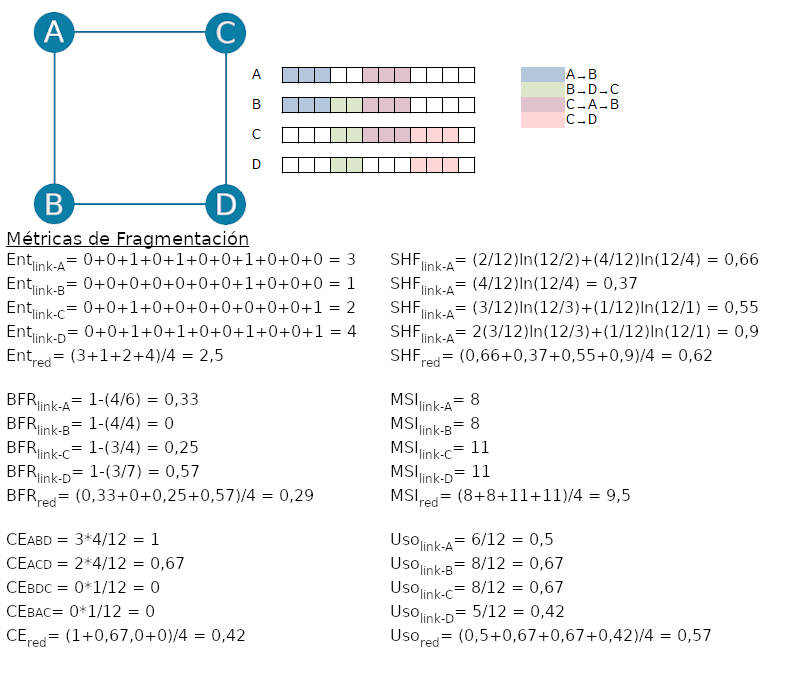
\includegraphics[width=1\textwidth]{capitulos/img/ejemploMetricasCompleto4.png}
    \caption{Ejemplo de métricas de fragmentación}
    \label{fig:ejemploMetricas}
\end{figure}

En la figura \ref{fig:ejemploMetricas} se puede ver un ejemplo de una topología con 4 conexiones activas, el estado de sus enlaces y el cálculo de cada una de las métricas de fragmentación explicadas anteriormente. 

\section{Obtención de datos para el entrenamiento}
Se utilizó un simulador de redes EON \cite{davalos2019spectrum} para la generación del conjunto de datos a ser utilizados para el entrenamiento de la red neuronal.

Para esto se utilizaron dos topologías de red: USNET y NSFNET, en donde por cada topología se realizaron 50 simulaciones con volumen de  tráfico variable en la misma simulación, para lograr que la cantidad de conexiones activas no permanezca constante durante la simulación.  La variación de tráfico usada fue la que se ve en la figura \ref{fig:traficos}-a, el proceso se realizó durante 1210 unidades de tiempo para cada simulación, generando un total de 121.000 registros.

Una vez generados los datos, los mismos fueron preprocesados, de forma a obtener los valores de la probabilidad de bloqueo que deseamos estimar.

El preprocesamiento consiste en el cálculo del índice de bloqueo en base a la ecuación \ref{eq:ecuacion_ib}, donde para un tiempo t, utilizando una ventana de 10 unidades de tiempo hacia delante, para cada instante podemos obtener una mirada hacia delante de posibles bloqueos, \(FSB_{i}\) es la sumatoria de \textit{FS} bloqueados en el tiempo \textit{i} y \(FSD_{i}\) es la sumatoria de \textit{FS} demandados en el tiempo \textit{i}.

\begin{equation} \label{eq:ecuacion_ib}
        PB_{t} = \frac{\sum_{i=t}^{t+T}FSB_{i}}{\sum_{i=t}^{t+T}FSD_{i}}
\end{equation}

Además, una vez separados los datos y debido a la diferencia de rangos de valores, los mismos son normalizados, usando la siguiente fórmula.
\begin{equation}
    n = x - \frac{train_{mean}}{train_{std}}
\end{equation}
Donde x es el valor que queremos normalizar, \(train_{mean}\) la media de valores y \(train_{std}\) es la desviación estándar. 

\begin{figure}
    \centering
    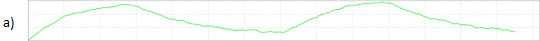
\includegraphics[width=1\textwidth]{capitulos/img/trafico_1_a.png}
    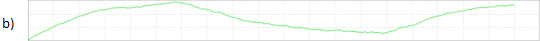
\includegraphics[width=1\textwidth]{capitulos/img/trafico_2_b.png}
    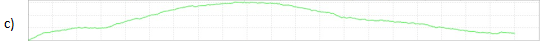
\includegraphics[width=1\textwidth]{capitulos/img/trafico_3_c.png}
    \caption{Volumen de tráfico variado utilizado}
    \label{fig:traficos}
\end{figure}

\section{Herramientas Utilizadas}

En esta sección se presentan las herramientas utilizadas para la implementación del método propuesto en este trabajo, seleccionadas luego de realizar numerosas ejecuciones de prueba para obtener los valores de los parámetros del modelo, asi como la prueba de concepto en sí.

Para todo el proceso de \textit{Machine Learning} se utilizó la plataforma de código abierto llamada \textit{\textbf{TensorFlow}} \cite{tensowFlow} en el lenguaje de programación \textit{\textbf{Python}}. En la creación y entrenamiento de redes neuronales se utilizó la API de alto nivel incluida en la plataforma \textit{\textbf{Tensorflow}} denominada \textit{\textbf{Keras}}, la cual permite la creación de modelos de aprendizaje automático de forma rápida y sencilla.

Elegimos Tensorflow como herramienta principal debido a que es una plataforma de código abierto orientado a \textit{Machine Learning}. Cuenta con un ecosistema completo de herramientas y librerías que facilitan la creación y desarrollo de aplicaciones de aprendizaje automático, además cuenta con una extensa y muy completa documentación.

\section{Modelado}

Para entrenar los datos recolectados se utilizó un modelo con una capa de entrada de 7 neuronas, dos capas ocultas densamente conectadas, cada una con 64 y 32 neuronas respectivamente, y una capa de salida que devuelve un único valor continuo.
Para todas las capas la función de activación utilizada fue la RELU (Ver sección 3.2.2).

\section{Entrenamiento}
Para el entrenamiento del modelo, se creó un conjunto de datos de entrenamiento utilizando el 70\% de los datos recolectados de forma aleatoria.  

El 20\% de los datos de entrenamiento se utilizó como el conjunto de validación. Una técnica utilizada en el procedimiento es el  llamado parada temprana o \textit{Early Stopping}, el cual mediante el monitoreo del rendimiento del entrenamiento nos permite detenernos una vez que el error de validación aumente de forma sostenida, de forma así evitar un sobre entrenamiento.

El modelo se entrena como máximo por 1000 épocas, el cual se detiene automáticamente cuando el valor del error de validación deja de mejorar. La figura \ref{fig:errorEpocas} muestra la evolución del error al pasar las épocas.

Los parámetros comparados son el error de entrenamiento o \textit{Train Error}, el cuál es el error obtenido durante la fase de entrenamiento del modelo y el error de validación o \textit{Val Error}, que se obtiene en la fase de validación.

Por cada época el \textit{Val Error} es comparado con el  \textit{Train Error},esto hasta que se determina que ya no existe mejora, sino que el error de validación se mantiene o aumenta su valor con respecto al punto de parada.


\begin{figure}[H]
    \centering
    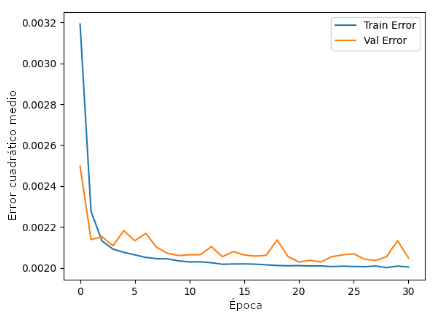
\includegraphics[width=9cm]{capitulos/img/graficoErrorEs.png}
    \caption{Evolución del error a través de épocas}
    \label{fig:errorEpocas}
\end{figure}

\section{Pruebas de predicción}
Para comprobar la efectividad de nuestro modelo se procedió a tomar el 30\% de datos restantes que no fueron incluidos en el entrenamiento y realizar predicciones, como ya conocemos el valor de la probabilidad de bloqueo que se busca predecir podemos calcular el error absoluto medio (MAE) y el error cuadrático medio (MSE). La tabla \ref{table:resultadosPrediccionTabla} muestra los resultados obtenidos, siendo éstos muy satisfactorios.

\begin{table}[H]
\centering
    \caption{Tabla de resultados en pruebas de predicción}
    \begin{tabular}{|l|l|}
        \hline
        MAE & 0.0239 \\ \hline
        MSE & 0.002  \\ \hline
    \end{tabular}
    \label{table:resultadosPrediccionTabla}
\end{table}
\newpage
\begin{figure}[H]
    \centering
    \begin{tabular}{@{}c@{}}
        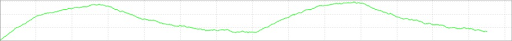
\includegraphics[width=1\textwidth]{capitulos/img/trafico_1.png}\\
        \small (a) Tráfico de volumen variable
    \end{tabular}
    \begin{tabular}{@{}c@{}}
        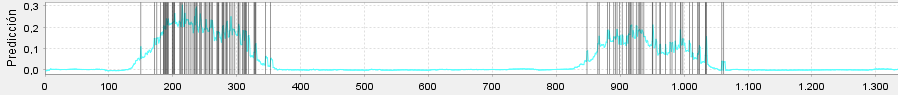
\includegraphics[width=1\textwidth]{capitulos/img/grafico_prediccion_usnet.PNG}\\
        \small (b) Gráfico de valores predichos por la red neuronal
    \end{tabular}
    \caption{Utilización de la red y predicciones}
    \label{fig:utilizacionPredicciones}
\end{figure}
En la Figura \ref{fig:utilizacionPredicciones} - a se observa la variación de la utilización de la red, al realizarse una simulación con volumen de tráfico variable sin realizar procesos de desfragmentación. En la parte b de la misma figura se observa la curva de valores predichos con las técnicas presentadas junto a los bloqueos dados en la misma simulación. Puede observarse cómo este valor acompaña la variación de la utilización de la red, y también toma valores más altos en periodos de tiempo en que la frecuencia de bloqueos se hace más alta. 
